\documentclass[11pt]{article}

\usepackage[T1]{fontenc}
\usepackage{lmodern}
\usepackage[margin=1.1in]{geometry}
\usepackage{amsmath,amssymb,amsthm}
\usepackage{booktabs}
\usepackage{array}
\usepackage{microtype}
\usepackage{xcolor}
\usepackage{graphicx}
\usepackage[font=small,labelfont=bf,width=0.95\textwidth]{caption}
\usepackage{placeins}
\usepackage{listings}
\usepackage[hidelinks]{hyperref}

\definecolor{codebg}{gray}{0.96}
\definecolor{codekw}{RGB}{0,90,160}
\definecolor{codecm}{RGB}{110,110,110}
\definecolor{codestr}{RGB}{150,60,20}

\lstset{
  language=Python,
  basicstyle=\ttfamily\footnotesize,
  keywordstyle=\color{codekw},
  commentstyle=\color{codecm}\itshape,
  stringstyle=\color{codestr},
  backgroundcolor=\color{codebg},
  frame=none,
  xleftmargin=1.2em,
  framexleftmargin=1.2em,
  aboveskip=1.0em,
  belowskip=1.0em,
  showstringspaces=false,
  breaklines=true,
  columns=fullflexible,
}

\theoremstyle{plain}
\newtheorem{proposition}{Proposition}
\newtheorem{lemma}{Lemma}
\newtheorem{theorem}{Theorem}
\newtheorem{corollary}{Corollary}
\theoremstyle{remark}
\newtheorem*{remark}{Remark}

% \code{} is \texttt, which cannot hyphenate; give TeX room in the narrower
% measure of the description lists rather than rewording around it.
\setlength{\emergencystretch}{2.5em}

% --- notation macros ---
\newcommand{\R}{\mathbb{R}}
\newcommand{\Mset}{\mathcal{M}}
\newcommand{\Sset}{\mathcal{S}}
\newcommand{\Kset}{\mathcal{K}}
\newcommand{\LN}{\mathrm{LN}}
\newcommand{\FFN}{\mathrm{FFN}}
\newcommand{\Attn}{\mathrm{Attn}}
\newcommand{\ip}[2]{\langle #1,\, #2\rangle}
\newcommand{\norm}[1]{\lVert #1 \rVert}
\newcommand{\code}[1]{\texttt{\small #1}}

\title{\textbf{An Exact Additive Decomposition of the MARINA \textsc{cls} Token}\\[0.4em]
\large Attributing the cross-attention read budget to input modalities}
\author{Anthony Tong}
\date{30 July 2026}

\begin{document}
\maketitle

\begin{abstract}
\noindent
MARINA's cross-attention stack reads from a memory that is constructed once and
never updated across blocks. This note shows that this single architectural
property makes the final \textsc{cls} token decompose \emph{exactly} into a sum
of per-source terms, and derives that decomposition in full: the span partition,
the source-wise split of multi-head attention, the linear transport of an
additive component through LayerNorm, and the resulting closed form for the
output. The decomposition induces a signed budget over sources that sums
identically to one --- the \emph{attribution}, or ``usage'', measure.
\S\ref{sec:budget}--\S\ref{sec:suppression} report the measured budget on three
trained seeds
($n = 23{,}648$ molecules each), set it against the \emph{ablation}, or
``irreplaceability'', measure obtained by withholding each modality, refine it
by depth into per-block \emph{injection} and \emph{survival}, and close with an
attention-suppression experiment. The final section states precisely where
exactness ends --- the feedforward nonlinearity and the input-dependence of the
attention weights --- and why that causal instrument is required at all.
Implementation references are to \code{src/modules/marina/model.py} on branch
\code{modality-attribution}; \S\ref{sec:provenance} separates what is
pre-existing trained-model code from what is measurement apparatus added for
this analysis.
\end{abstract}

\newpage
\setcounter{tocdepth}{2}
{\parskip 0pt \tableofcontents}
\newpage

\section{Vocabulary}
\label{sec:vocab}

Six terms are used throughout in a specific sense. Three name things that exist
in the trained model; three name things the measurement introduces.

\medskip
\noindent\textbf{In the model.}

\begin{description}\setlength{\itemsep}{4pt}
  \item[Memory] The matrix $M$ that the global \textsc{cls} query reads from:
    every modality's encoded tokens, concatenated into one sequence. Built once
    per forward pass by \code{\_encode} and never modified afterwards.
  \item[Segment] The contiguous block of memory rows belonging to one modality.
    Modality $m$'s segment has $L_m$ rows: one mod-token followed by $L_m - 1$
    peak rows. \code{\_encode} returns the layout as
    \code{segments = [(m, $L_m$), \dots]}.
  \item[Mod-token] A learned per-modality vector $\tau_m$, an
    \code{nn.Parameter} held in \code{self.mod\_tokens}, prepended as the
    \emph{first} row of modality $m$'s segment. It is a ``this modality is
    present'' marker, playing the role a segment embedding plays in BERT. It is
    part of the trained model, not of this analysis. See
    \S\ref{sec:modtoken}.
\end{description}

\medskip
\noindent\textbf{In the measurement.}

\begin{description}\setlength{\itemsep}{4pt}
  \item[Span] An index set $\Sset_k$ over memory rows, used to group rows that
    should be credited together. Spans exist only in the instrumentation; the
    model has no notion of them.
  \item[Bucket] A named additive term in the decomposition of the final
    \textsc{cls}. Each span yields one bucket, and there are three further
    buckets for things no span can own (\code{ffn}, \code{bias},
    \code{cls\_init}). Table~\ref{tab:buckets} is the full inventory.
  \item[Contribution] The vector $c_k \in \R^d$ that bucket $k$ adds to the
    final \textsc{cls}. Its scalar \emph{share} is the projection
    \eqref{eq:share} of that vector onto the output direction.
\end{description}

\medskip
\noindent
Four measures are then built on these, and are easy to conflate:
\emph{attribution} (usage --- share of what is read, everything present),
\emph{ablation} (irreplaceability --- cosine lost when a modality is withheld),
\emph{injection} (the norm of a contribution where it was written), and
\emph{survival} (how much of that contribution reaches the output). The first
two are compared in \S\ref{sec:budget}, the second two defined in
\S\ref{sec:depth}.

\section{What is pre-existing and what is instrumentation}
\label{sec:provenance}

Three tiers of code appear in this note, and it matters which is which: only
the first two ran during training and produced the weights being analysed.
\emph{Nothing in tier~3 participates in training, inference, or the loss.} It
is read-only apparatus, added on branch \code{modality-attribution} in a commit
that is \textbf{+175/$-$4} lines on \code{model.py} --- and the four deleted
lines are only \code{forward}'s encoder body being extracted verbatim into
\code{\_encode} so the instrumentation can reuse it.

\begin{table}[htbp]
\centering
\small
\caption{Provenance. Tier 3 is measurement apparatus; it changes no weights and
alters no forward pass.}
\label{tab:provenance}
\renewcommand{\arraystretch}{1.15}
\begin{tabular}{@{}l l p{5.3cm}@{}}
\toprule
Tier & Symbol & What \\
\midrule
\textbf{1. Stock PyTorch}
  & \code{nn.MultiheadAttention} & the cross-attention layer itself; defined in
    \S\ref{sec:attn} \\
  & \code{nn.LayerNorm} & defined in \S\ref{sec:ln} \\
  & \code{nn.TransformerEncoder} & the per-modality self-attention in
    \code{\_encode} \\
\addlinespace
\textbf{2. MARINA, pre-existing}
  & \code{CrossAttentionBlock.forward} & the trained path: one block of
    attention $\to$ LN $\to$ FFN $\to$ LN \\
  & \code{MARINA.forward} & the full stack; what training and evaluation call \\
  & \code{\_encode} & builds $M$; extracted from \code{forward}, behaviour
    unchanged \\
\addlinespace
\textbf{3. Instrumentation (new)}
  & \code{attn\_contributions} & splits one block's attention output by span
    (Prop.~\ref{prop:split}) \\
  & \code{forward\_contributions} & the full decomposition
    (Thm.~\ref{thm:main}) \\
  & \code{\_ln\_component}, \code{\_ln\_sigma} & transports one component
    through a LayerNorm (Lem.~\ref{lem:ln}) \\
\bottomrule
\end{tabular}
\end{table}

\noindent
The distinction is not bookkeeping pedantry. The equations in
\S\ref{sec:attn} and \S\ref{sec:ln} describe what \emph{stock PyTorch} computes;
the propositions about them are claims that the instrumentation reproduces that
computation exactly, and each is checkable against the stock layer's own
output. Where a code listing follows, its first line states its tier.

\section{Notation}

Everything below is written \emph{per sample}; the batch axis is suppressed,
since no operation in the stack mixes across it. Vectors are column vectors in
$\R^d$.

\begin{center}
\footnotesize
\renewcommand{\arraystretch}{1.2}
\begin{tabular}{@{}l l l@{}}
\toprule
\textbf{Symbol} & \textbf{Meaning} & \textbf{Code} \\
\midrule
$d$ & model width & \code{args.dim\_model} \\
$H$ & attention heads; $d_h = d/H$ & \code{args.heads} \\
$N$ & cross-attention blocks ($N=16$) & \code{len(self.cross\_blocks)} \\
$\ell \in \{0,\dots,N-1\}$ & block index & \code{li} \\
$\Mset$ & modality set, $\lvert\Mset\rvert = 5$ & \code{args.input\_types} \\
$L_m$ & segment length of modality $m$ (peaks $+$ mod-token) & \code{L + 1} \\
$L$ & total memory length, $L = \sum\nolimits_m L_m$ & \code{joint\_seq.size(1)} \\
$M \in \R^{L\times d}$ & joint memory, rows $M_j$ & \code{joint\_seq} \\
$\pi \in \{0,1\}^L$ & key-padding mask & \code{joint\_mask} \\
$q_\ell \in \R^d$ & \textsc{cls} state entering block $\ell$ & \code{global\_token} \\
$g \in \R^d$ & learned initial \textsc{cls} query & \code{self.global\_cls} \\
$\tau_m \in \R^d$ & learned mod-token of modality $m$ & \code{self.mod\_tokens[m]} \\
$W_Q, W_K, W_V \in \R^{d\times d}$, $b_V$ & attention in-projections & \code{attn.in\_proj\_*} \\
$W_O \in \R^{d\times d}$, $b_O$ & attention out-projection & \code{attn.out\_proj} \\
$\gamma^{(i)}_\ell, \beta^{(i)}_\ell \in \R^d$ & LayerNorm gain / bias, $i\in\{1,2\}$ & \code{norm1}, \code{norm2} \\
$\varepsilon$ & LayerNorm epsilon & \code{norm.eps} \\
\bottomrule
\end{tabular}
\end{center}

\medskip
\noindent
We use $\gamma,\beta$ for the LayerNorm parameters, following Ba et
al.~(2016), and reserve $\alpha$ for attention weights. The frozen-scale
linearisation of LayerNorm in Section~\ref{sec:ln} is the standard device from
Elhage et al., \emph{A Mathematical Framework for Transformer Circuits}
(2021); there it is used to fold LayerNorm into adjacent linear maps, whereas
here it is used to push a sum through it componentwise.

\section{The static-memory property}
\label{sec:static}

This is the structural precondition for everything that follows.

\begin{lstlisting}
# --- Tier 3: forward_contributions. The tier-2 forward() has the same shape:
# one _encode, then a loop over cross_blocks reusing the same joint_seq.
joint_seq, joint_mask, segments = self._encode(batch)   # model.py:296 -- once
for li, block in enumerate(self.cross_blocks):
    parts, attn_out = block.attn_contributions(
        global_token, joint_seq, joint_mask, spans)
\end{lstlisting}

\noindent
The memory $M$ is built once and passed unchanged to all $N$ blocks; only
$q_\ell$ evolves. There is \emph{no} self-attention over $M$ between blocks, so
a memory row never mixes with rows outside its own segment during the
cross-attention stack.

\begin{remark}[What is and is not pure]
Inside \code{\_encode}, each modality \emph{does} receive a self-attention
stack --- but a \emph{separate one per modality}, applied before concatenation
(\code{model.py:239}). Consequently row $M_j$ in segment $m$ is a mixture of
modality $m$'s own peaks and $\tau_m$, and of nothing else. Purity therefore
holds at the \emph{modality} level, which is the level at which the
decomposition makes claims. It does \emph{not} hold at the level of individual
peaks: one cannot attribute the final \textsc{cls} to peak $\#7$ of the HSQC
spectrum by this construction.
\end{remark}

\noindent
In a standard encoder--decoder or decoder-only stack the construction fails
outright, because the memory (respectively, the residual stream) mixes sources
at every layer.

\section{The span partition}

Let $o_m$ denote the offset of segment $m$ in the concatenation. Define index
sets $\Sset_k \subseteq \{1,\dots,L\}$ (\code{model.py:299--308}):
\[
  \Sset_{m:\text{token}} = \{o_m\},
  \qquad
  \Sset_{m} = \{o_m+1,\ \dots,\ o_m + L_m - 1\}.
\]

\begin{proposition}[Completeness]
\label{prop:partition}
The family $\{\Sset_k\}_{k \in \Sset}$, where
$\Sset = \Mset \cup \{m{:}\text{token}\}_{m\in\Mset}$, is a \emph{partition} of
$\{1,\dots,L\}$: pairwise disjoint and exhaustive.
\end{proposition}

\noindent
This is what makes the split of Section~\ref{sec:attn} exact rather than
approximate --- no position is double-counted and none is dropped. For five
modalities, $\lvert\Sset\rvert = 10$ spans, hence ten source buckets.

\subsection{The bucket inventory}

\begin{table}[htbp]
\centering
\small
\caption{The thirteen aggregate buckets, with their seed-1 shares. Every one
is a vector $c_k \in \R^d$; the share is its projection \eqref{eq:share}. They
sum to $1$ by Corollary~\ref{cor:budget}. (Theorem~\ref{thm:main} indexes each
source bucket by block as well, giving $178$ before summing over $\ell$.)}
\label{tab:buckets}
\renewcommand{\arraystretch}{1.15}
\begin{tabular}{@{}l c p{6.1cm} r@{}}
\toprule
Bucket & Count & What the \textsc{cls} read it from & Share \\
\midrule
$m$ & 5 & modality $m$'s \emph{peak} rows --- the actual spectrum & 0.2324 \\
$m{:}\text{token}$ & 5 & modality $m$'s \emph{mod-token} row alone & 0.0071 \\
\code{ffn} & 1 & nothing --- written by the feedforward path & 0.7199 \\
\code{bias} & 1 & nothing --- $b_O$, $\beta^{(1)}$, $\beta^{(2)}$ & 0.0406 \\
\code{cls\_init} & 1 & nothing --- the learned initial query $g$ & $\approx 0$ \\
\midrule
& 13 & & 1.0000 \\
\bottomrule
\end{tabular}
\end{table}

\noindent
Only the first row is ``information read off the spectra''. The naming in the
results tables follows this: Table~\ref{tab:budget}'s \emph{Share} column is
the $m$ bucket alone, its \emph{Mod-token} column is the $m{:}\text{token}$
bucket, and \emph{Peaks-only} renormalises the five $m$ buckets to sum to one.

\subsection{What the \texorpdfstring{$m{:}\text{token}$}{m:token} bucket is}
\label{sec:modtoken}

This bucket is the one most easily misread, so it is worth being explicit.

Each modality's segment is $[\,\tau_m,\ \text{peak}_1,\ \dots,\
\text{peak}_{L_m-1}\,]$ --- the learned mod-token first, then the encoded
peaks. The instrumentation cuts each segment into \emph{two} spans rather than
one: the single row $\{o_m\}$ holding $\tau_m$, and the $L_m - 1$ rows holding
the peaks. So for HSQC there are two buckets: \code{hsqc}, what the \textsc{cls}
read off actual HSQC cross-peaks, and \code{hsqc:token}, what it read off the
marker row.

\paragraph{Why split them.} When a modality is withheld, every one of its peak
rows is masked (\code{mask = (x.abs().sum(-1) == 0)}, \code{model.py:234}), so
$\alpha_j = 0$ there and the $m$ bucket is \emph{exactly} zero. The
$m{:}\text{token}$ bucket is not: the marker row is never masked. Keeping them
apart therefore separates \emph{reliance on the spectrum} from \emph{reliance
on knowing the spectrum was supplied}. Collapsed into one bucket, a modality
that is merely announced would look partly used.

\paragraph{What it is worth.} Together the five mod-token buckets take
$0.0071$ of the budget on seed 1 --- under $1\%$, and about $3\%$ of what the
peak buckets take. Individually they run from $-0.0004$
(\code{mass\_spec:token}, which pulls slightly \emph{against} the output
direction) to $+0.0027$ (\code{hsqc:token}). The exception is \code{mw}, whose
mod-token share ($+0.0021$) equals its peak share ($+0.0021$) --- half of
what molecular weight contributes is the bare fact that it was provided.

\begin{remark}[The bucket is not a clean ``presence prior'' in general]
$\tau_m$ is prepended \emph{before} modality $m$'s self-attention stack runs
(\code{model.py:237--239}), so when peaks are present the marker row absorbs
information from them. The $m{:}\text{token}$ bucket is then the mod-token
position \emph{after} that mixing, not the learned parameter in isolation. It
is a clean presence prior only in the absent case, where the peak rows are all
masked and the marker attends to itself alone. Read the modality-present
mod-token shares as ``what the \textsc{cls} took from the segment's summary
row'', not as ``the value of the prior''.
\end{remark}

\section{Attention splits exactly by source}
\label{sec:attn}

\subsection{What \texorpdfstring{\code{nn.MultiheadAttention}}{nn.MultiheadAttention} computes}
\label{sec:mha}

\emph{Tier 1 --- stock PyTorch.} Everything in this subsection is the standard
layer's own definition, not MARINA code and not instrumentation. Each
\code{CrossAttentionBlock} owns one such layer, constructed
\code{nn.MultiheadAttention(embed\_dim=$d$, num\_heads=$H$, bias=True,
batch\_first=True)}.

The layer holds its three input projections \emph{packed} into one
$3d \times d$ parameter \code{in\_proj\_weight} (rows $0{:}d$ for $W_Q$,
$d{:}2d$ for $W_K$, $2d{:}3d$ for $W_V$) with \code{in\_proj\_bias} packed the
same way, plus a separate \code{out\_proj} carrying $W_O$ and $b_O$. Given a
query and a key/value sequence it projects both, splits the width into $H$
heads of size $d_h = d/H$, forms scaled dot-product attention per head with
masked positions driven to $-\infty$ before the softmax, takes the
value-weighted sum, concatenates the heads and applies \code{out\_proj}.
Dropout is applied to the attention weights in training only; here the model is
in \code{eval()} and \code{forward\_contributions} is
\code{@torch.no\_grad()}, so it is inactive.

MARINA's trained path calls this layer once per block and keeps only its
output:

\begin{lstlisting}
# --- Tier 2: MARINA, pre-existing. This is the path that trained the weights.
attn_out, _ = self.attn(query, key, value,
                        key_padding_mask=key_padding_mask,
                        need_weights=False)      # <- weights discarded
q1 = self.norm1(query + attn_out)
out = self.norm2(q1 + self.ff(q1))
\end{lstlisting}

\noindent
Written out, with a single query (the \textsc{cls}), the layer computes the
following. Write $\alpha^{(h,\ell)} \in \R^L$ for the attention row of head $h$
at block $\ell$:
\[
  \alpha^{(h,\ell)}_j
  = \frac{\exp\!\big(\ip{W_Q^{(h)} q_\ell}{W_K^{(h)} M_j} / \sqrt{d_h}\big)\,
          \mathbf{1}[\pi_j = 0]}
         {\sum_{j'} \exp\!\big(\ip{W_Q^{(h)} q_\ell}{W_K^{(h)} M_{j'}} / \sqrt{d_h}\big)\,
          \mathbf{1}[\pi_{j'} = 0]},
  \qquad
  \sum_{j=1}^{L} \alpha^{(h,\ell)}_j = 1,
\]
with values $v^{(h)}_j = W_V^{(h)} M_j + b_V^{(h)}$. The block's attention
output is
\begin{equation}
  a_\ell \;=\; \sum_{h=1}^{H} \sum_{j=1}^{L}
    \alpha^{(h,\ell)}_j\, W_O^{(h)} v^{(h)}_j \;+\; b_O .
  \label{eq:attn}
\end{equation}

\noindent
Equation~\eqref{eq:attn} is a restatement of the stock layer; nothing has been
added yet. The key structural fact it exposes --- the one the next subsection
exploits --- is that the output is a \textbf{sum over source positions $j$}.

\subsection{How the instrumentation splits it}

\emph{Tier 3 --- new.} \code{attn\_contributions} is a second, read-only entry
point on \code{CrossAttentionBlock}. It does not replace
\code{CrossAttentionBlock.forward} and is never called by it; the trained path
above is untouched.

\begin{proposition}[Exact source-wise split]
\label{prop:split}
Define, for each bucket $k \in \Sset$,
\begin{equation}
  \boxed{\;
  p_{k,\ell} \;=\; \sum_{h=1}^{H} \sum_{j \in \Sset_k}
    \alpha^{(h,\ell)}_j\, W_O^{(h)} v^{(h)}_j \; }
  \label{eq:parts}
\end{equation}
Then $\sum_{k \in \Sset} p_{k,\ell} + b_O = a_\ell$ identically.
\end{proposition}

\begin{proof}
The outer sum over $j$ in \eqref{eq:attn} is a plain sum, and by
Proposition~\ref{prop:partition} the sets $\{\Sset_k\}$ partition its index
range. Regrouping the terms is therefore an identity.
\end{proof}

\noindent
In code (\code{model.py:93--110}), abridged:

\begin{lstlisting}
# --- Tier 3: instrumentation. Read-only; not on the trained path.
# Same stock layer as forward() calls -- the only change is need_weights.
attn_out, alpha = self.attn(query, kv, kv, key_padding_mask=key_padding_mask,
                            need_weights=True, average_attn_weights=False)
alpha = alpha[:, :, 0, :]                              # (B, H, L); one query

# Re-derive the value projection: rows 2E: of the packed in_proj ARE W_V, b_V.
v = F.linear(kv, self.attn.in_proj_weight[2 * E:], self.attn.in_proj_bias[2 * E:])
v = v.view(B, L, H, hd).permute(0, 2, 1, 3)            # (B, H, L, hd)

for name, sel in spans.items():
    o = torch.einsum('bhl,bhld->bhd', alpha[:, :, sel], v[:, :, sel])
    parts[name] = F.linear(o.reshape(B, E), self.attn.out_proj.weight)
return parts, attn_out          # attn_out is the stock layer's own output
\end{lstlisting}

\noindent
Three things to note. The \code{einsum} contracts over the selected positions
$\Sset_k$ and the head dimension, and \code{F.linear} \emph{without} a bias
argument applies $W_O$ to the concatenated heads, which is exactly
$\sum_h W_O^{(h)}(\cdot)^{(h)}$; $b_O$ is deliberately excluded and routed to
the \code{bias} bucket at \code{model.py:332}. Masked positions carry
$\alpha_j = 0$, so an absent modality's peak bucket is exactly zero. And the
function returns \code{attn\_out} --- the \emph{stock} layer's output --- next
to the hand-computed \code{parts}, so Proposition~\ref{prop:split} is not an
assumption about PyTorch's internals but a claim that can be, and is, checked
against them.

\begin{remark}[Why the value projection is recomputed]
\code{nn.MultiheadAttention} returns the attention weights but not the
per-position values, and the weighted sum over $j$ happens inside the fused
kernel. Splitting by source therefore requires re-deriving $v$ outside the
layer. Slicing rows $2d{:}3d$ of \code{in\_proj\_weight} is not an
approximation --- that block \emph{is} $W_V$, by the layer's own packing
convention (\S\ref{sec:mha}) --- but it is a coupling to that convention, and
it is the one place where the instrumentation reaches into stock internals
rather than calling a documented interface.
\end{remark}

\begin{remark}[Two caveats at this step]
\emph{(i) The weights $\alpha$ are softmax-coupled.} The quantity $p_{k,\ell}$
decomposes the output \emph{given the realised attention pattern}. It is not
the counterfactual ``what if $\Sset_k$ were absent'': removing a span
renormalises $\alpha$ over the survivors. This is the formal reason attribution
and ablation are distinct measures.

\emph{(ii) The value bias $b_V$ is apportioned, not isolated.} Since
$v^{(h)}_j$ includes $b_V^{(h)}$ and $\sum_j \alpha_j = 1$, the value bias
contributes $\sum_h W_O^{(h)} b_V^{(h)}$ in total, divided among buckets in
proportion to their attention mass. Unlike $b_O$ it is not separated out.
Being source-independent, it slightly inflates high-attention buckets. With the
\code{bias} bucket at $0.041$ of the budget against $0.72$ for the feedforward
term this is second-order, but it is a genuine approximation inside an
otherwise exact split.
\end{remark}

\section{LayerNorm is linear in the components of its input}
\label{sec:ln}

\emph{Tier 1 --- stock PyTorch.} \code{nn.LayerNorm} normalises each vector
over its feature dimension and then applies a learned elementwise gain and
bias: $\LN_{\gamma,\beta}(z) = \gamma \odot (z - \mu(z))/\sigma(z) + \beta$,
with $\mu$ and $\sigma$ the mean and standard deviation \emph{of $z$ itself}.
Each \code{CrossAttentionBlock} owns two, \code{norm1} after attention and
\code{norm2} after the feedforward; $\gamma$ and $\beta$ are trained
parameters. This section establishes a property of that stock layer; the
tier-3 helper \code{\_ln\_component} then applies it.

Let $C = I_d - \tfrac{1}{d}\mathbf{1}\mathbf{1}^{\!\top}$ be the centering
projector and
\[
  \sigma(z) \;=\; \sqrt{\tfrac{1}{d}\norm{Cz}_2^2 + \varepsilon},
\]
which is \code{\_ln\_sigma}; note \code{var(..., unbiased=False)} equals
$\tfrac1d\norm{Cz}^2$ exactly. Then
$\LN_{\gamma,\beta}(z) = \gamma \odot Cz/\sigma(z) + \beta$. For a
\emph{fixed} scalar $s > 0$ define the linear operator
\begin{equation}
  \boxed{\;A_{\gamma,s} \;:=\; \tfrac{1}{s}\,\mathrm{diag}(\gamma)\,C
  \;\in\; \R^{d\times d}.\;}
  \label{eq:lnop}
\end{equation}

\begin{lemma}[Component transport]
\label{lem:ln}
For any decomposition $z = \sum_k c_k$,
\[
  \LN_{\gamma,\beta}(z) \;=\; \sum_k A_{\gamma,\sigma(z)}\, c_k \;+\; \beta .
\]
\end{lemma}

\begin{proof}
$A_{\gamma,\sigma(z)}$ is linear, so
$\sum_k A_{\gamma,\sigma(z)} c_k = A_{\gamma,\sigma(z)} \sum_k c_k
= A_{\gamma,\sigma(z)} z = \gamma \odot Cz / \sigma(z)$. Adding $\beta$ once
gives $\LN_{\gamma,\beta}(z)$.
\end{proof}

\noindent
The entire content of the lemma is that $\sigma$ is evaluated on the
\emph{full} $z$ and then held fixed. The only nonlinearity in LayerNorm is the
scalar $\sigma(\cdot)$; freezing it makes the map exactly linear on that
forward pass. This is why the implementation threads \code{sigma} in from
outside rather than recomputing it per component:

\begin{lstlisting}
# --- Tier 3: instrumentation helper.
def _ln_component(ln, c, sigma):
    # sigma must be computed from the full z, not from c
    return ln.weight * (c - c.mean(-1, keepdim=True)) / sigma
\end{lstlisting}

\begin{remark}
$A_{\gamma,\sigma(z)}$ is a \emph{data-dependent} linear map. It is not the
Jacobian of $\LN$, and Lemma~\ref{lem:ln} does not linearise $\LN$ as a
function --- it is a statement about one realised forward pass. The
requirement that $\beta$ be added exactly once is also why \code{bias} must be
its own bucket: mapping every component through $\LN$ naively would add $\beta$
once per bucket.
\end{remark}

\section{The block recursion and transport operators}

Block $\ell$ (\code{model.py:326--348}), with $q_0 = g$:
\[
\begin{aligned}
  z^{(1)}_\ell &= q_\ell + a_\ell, &
  s^{(1)}_\ell &= \sigma\big(z^{(1)}_\ell\big), &
  u_\ell &= \LN^{(1)}_\ell\big(z^{(1)}_\ell\big), \\[2pt]
  f_\ell &= \FFN_\ell(u_\ell), & & & & \\[2pt]
  z^{(2)}_\ell &= u_\ell + f_\ell, &
  s^{(2)}_\ell &= \sigma\big(z^{(2)}_\ell\big), &
  q_{\ell+1} &= \LN^{(2)}_\ell\big(z^{(2)}_\ell\big).
\end{aligned}
\]
Residual addition distributes over buckets trivially. Writing
$A^{(i)}_\ell := A_{\gamma^{(i)}_\ell,\, s^{(i)}_\ell}$ as in \eqref{eq:lnop},
define the \emph{block transport}
\[
  \Psi_\ell \;=\; A^{(2)}_\ell A^{(1)}_\ell,
  \qquad
  \Psi_{>\ell} \;=\; \Psi_{N-1}\Psi_{N-2}\cdots\Psi_{\ell+1}
  \quad (\Psi_{>N-1} = I).
\]
There are three injection points, hence three transports to the output:

\begin{center}
\begin{tabular}{@{}l l l@{}}
\toprule
\textbf{Injected at} & \textbf{Passes through} & \textbf{Operator} \\
\midrule
$g$, before block $0$ & all blocks $0,\dots,N-1$
  & $T^{\text{init}} = \Psi_{N-1}\cdots\Psi_0$ \\
attention of block $\ell$ & $A^{(1)}_\ell$, $A^{(2)}_\ell$, then blocks $>\ell$
  & $T^{\mathrm a}_\ell = \Psi_{>\ell}\,\Psi_\ell$ \\
feedforward of block $\ell$ & $A^{(2)}_\ell$, then blocks $>\ell$
  & $T^{\mathrm f}_\ell = \Psi_{>\ell}\,A^{(2)}_\ell$ \\
\bottomrule
\end{tabular}
\end{center}

\medskip
\noindent
These operators are never materialised as matrices. The \code{stack} tensor of
shape $(\lvert\Kset\rvert, B, 1, d)$ holds every bucket's current value, and a
single broadcast call to \code{\_ln\_component} advances all of them one step
(\code{model.py:336, 346}). Buckets for blocks not yet reached hold zeros, and
$A_{\gamma,s}\mathbf{0} = \mathbf{0}$, so preallocating the full set is safe.

\begin{theorem}[Exact additive decomposition]
\label{thm:main}
\[
  q_N \;=\;
  \underbrace{T^{\text{init}} g}_{\code{cls\_init}}
  \;+\; \sum_{\ell=0}^{N-1}\sum_{k\in\Sset}
        \underbrace{T^{\mathrm a}_\ell\, p_{k,\ell}}_{\code{(k,$\,\ell$)}}
  \;+\; \sum_{\ell=0}^{N-1}
        \underbrace{T^{\mathrm f}_\ell\, f_\ell}_{\code{(ffn,$\,\ell$)}}
  \;+\; \underbrace{\sum_{\ell=0}^{N-1}
        \Big[T^{\mathrm a}_\ell b_O^{(\ell)}
           + T^{\mathrm f}_\ell \beta^{(1)}_\ell
           + \Psi_{>\ell}\,\beta^{(2)}_\ell\Big]}_{\code{bias}}
\]
\end{theorem}

\begin{proof}
Induction on $\ell$. Proposition~\ref{prop:split} splits $a_\ell$ into
per-source terms plus $b_O$; Lemma~\ref{lem:ln} pushes the accumulated sum
through each LayerNorm while adding each $\beta$ exactly once; residual
additions distribute. Composing the per-block maps gives the stated
transports.
\end{proof}

\noindent
The three transports of the bias term correspond exactly to the three
\code{+=} sites and their placement relative to the \code{\_ln\_component}
calls:

\begin{lstlisting}
# --- Tier 3: inside forward_contributions.
stack[bias_i] += block.attn.out_proj.bias   # before A1  -> gets T^a
...  stack = _ln_component(block.norm1, stack, sigma1)
stack[bias_i] += block.norm1.bias           # after A1   -> gets T^f
...  stack = _ln_component(block.norm2, stack, sigma2)
stack[bias_i] += block.norm2.bias           # after A2   -> gets Psi_{>l}
\end{lstlisting}

\noindent
Moving any one of those lines across an \code{\_ln\_component} call silently
breaks the identity of Theorem~\ref{thm:main}.

\paragraph{Bucket count.}
\[
  \lvert\Kset\rvert
  = \underbrace{2}_{\text{init, bias}}
  + N\cdot\big(\underbrace{2\lvert\Mset\rvert}_{\text{spans}}
             + \underbrace{1}_{\text{ffn}}\big)
  = 2 + 16\cdot 11 = 178 .
\]
The aggregate contributions sum over $\ell$ (\code{model.py:351--354}),
collapsing $178$ buckets to $13$: five modalities, five \code{:token} buckets,
plus \code{ffn}, \code{cls\_init} and \code{bias}. The $176$ per-layer entries
recorded in \code{perlayer\_seed1\_n256.json} are the $N\cdot 11$ terms.

\section{From vectors to a budget that sums to one}

Theorem~\ref{thm:main} yields $178$ \emph{vectors}. To obtain scalars, project
onto the output direction $\hat q_N = q_N / \norm{q_N}$ and normalise once more
by $\norm{q_N}$:
\begin{equation}
  \boxed{\;
  \text{share}_k
  \;=\; \frac{\ip{c_k}{\hat q_N}}{\norm{q_N}}
  \;=\; \frac{\ip{c_k}{q_N}}{\norm{q_N}^2}\;}
  \label{eq:share}
\end{equation}

\begin{corollary}
\label{cor:budget}
$\displaystyle\sum_{k\in\Kset}\text{share}_k = 1$.
\end{corollary}

\begin{proof}
$\sum_k \ip{c_k}{q_N} / \norm{q_N}^2
 = \ip{\sum_k c_k}{q_N} / \norm{q_N}^2
 = \norm{q_N}^2 / \norm{q_N}^2 = 1$,
using Theorem~\ref{thm:main} for the middle equality.
\end{proof}

\noindent
Two properties of \eqref{eq:share} are worth stating explicitly.

\begin{itemize}
  \item It is \emph{signed}. A bucket with $\ip{c_k}{q_N} < 0$ receives a
        negative share, meaning it pulls against the output direction.
  \item It is a \emph{scalar projection}: $\text{share}_k\norm{q_N}$ is the
        length of $c_k$'s component along $q_N$, and the orthogonal component
        of $c_k$ is discarded. A bucket may be large in norm and score
        approximately zero by being orthogonal to $q_N$. The double
        normalisation is what makes the quantity dimensionless and additive to
        one, rather than a cosine, which would not sum.
\end{itemize}

\paragraph{Numerical verification.}
Over $n = 23{,}648$ test molecules (seed 1), the implementation reports
$\sum_k \text{share}_k = 1.0000000119$ and
$\text{share}_{\code{cls\_init}} = -3.06\times 10^{-19}$. The first figure is
the integration test for
Propositions~\ref{prop:partition}--\ref{prop:split},
Lemma~\ref{lem:ln} and Theorem~\ref{thm:main} jointly: any error in the
partition, in the threading of $\sigma$, or in the placement of the bias
updates breaks it. The second says that after sixteen LayerNorms the learned
initial query contributes nothing whatsoever to the final \textsc{cls}; it
functions purely as a seed for the first attention.

\section{Results: the modality budget}
\label{sec:budget}

All figures below are measured on the three \code{marina-final-run} seed
checkpoints, $n = 23{,}648$ test molecules each, with all five modalities
present (mean \code{all\_inputs} cosine $0.9547$).

\begin{table}[htbp]
\centering
\small
\caption{The measured budget. \emph{Share} is \eqref{eq:share} over the whole
budget; \emph{peaks-only} renormalises over the five modality buckets, and is
the column to use for comparing modalities. \emph{Mod-token} is the
$m{:}\text{token}$ bucket. The first four columns are means over three seeds;
ablation drops are given per seed.}
\label{tab:budget}
\begin{tabular}{@{}l r r r r l@{}}
\toprule
Modality & Share & Peaks-only & Mod-token & Live tokens & Ablation drop (s0 / s1 / s2) \\
\midrule
HSQC & 0.1038 & \textbf{0.4474} & +0.0038 & 22.6 & 0.0130 / 0.0124 / 0.0127 \\
$^{13}$C NMR & 0.0589 & 0.2539 & +0.0016 & 25.6 & 0.0056 / 0.0056 / 0.0058 \\
MS & 0.0393 & 0.1692 & +0.0003 & 33.6 & 0.0054 / 0.0067 / 0.0067 \\
$^{1}$H NMR & 0.0279 & 0.1204 & +0.0016 & 25.3 & 0.0037 / 0.0034 / 0.0033 \\
MW & 0.0021 & 0.0092 & +0.0021 & 1.0 & 0.0006 / 0.0007 / 0.0006 \\
\bottomrule
\end{tabular}
\end{table}

\begin{table}[htbp]
\centering
\small
\caption{The three buckets that are not attributable to a source. Together
with the five modality and five mod-token buckets these complete the budget of
Corollary~\ref{cor:budget}.}
\label{tab:unattributed}
\begin{tabular}{@{}l r r r r@{}}
\toprule
Bucket & Seed 0 & Seed 1 & Seed 2 & Mean \\
\midrule
\code{ffn} & 0.71217 & 0.71991 & 0.70859 & \textbf{0.71355} \\
\code{bias} & 0.04510 & 0.04064 & 0.04950 & 0.04508 \\
\code{cls\_init} & $-6.7\times10^{-21}$ & $-3.1\times10^{-19}$ & $-3.5\times10^{-25}$ & $\approx 0$ \\
\bottomrule
\end{tabular}
\end{table}

\begin{figure}[htbp]
\centering
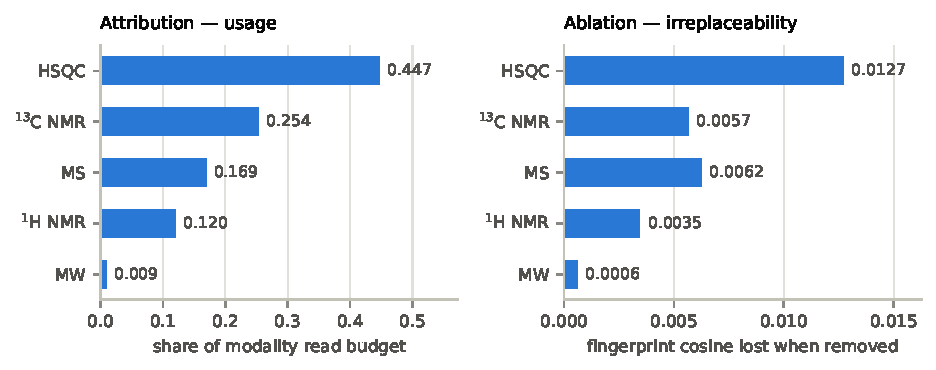
\includegraphics[width=\textwidth]{fig-usage-vs-irreplaceability.pdf}
\caption{Usage against irreplaceability, mean over three seeds. The two
measures are on different scales by roughly $30\times$, so they are shown as
two panels rather than one chart with two axes; the category order is fixed by
attribution in both. The rankings agree except for one adjacent swap
($^{13}$C NMR and MS), and the magnitudes do not agree at all.}
\label{fig:usage}
\end{figure}

Three observations.

\begin{enumerate}
  \item \textbf{The feedforward path dominates.} Only about $23\%$ of the final
        \textsc{cls} direction comes from modality tokens at all;
        $0.714$ is written by the feedforward path and $0.045$ by biases. This
        is why Table~\ref{tab:budget}'s peaks-only column, not its share
        column, is the meaningful cross-modality comparison.
  \item \textbf{HSQC dominates by both measures} --- $45\%$ of the peaks-only
        budget and the largest ablation drop --- consistent with ME-HSQC being
        the strongest single modality in the SPECTRE results.
  \item \textbf{The two measures agree on order and disagree on scale.} HSQC
        carries $45\%$ of the read budget, yet removing it costs $0.013$
        cosine. Spearman's $\rho$ between the peaks-only share and the ablation
        drop is $1.0$, $0.9$, $0.9$ across seeds 0--2; on seeds 1 and 2 the
        single adjacent swap is $^{13}$C NMR against MS.
\end{enumerate}

\noindent
The disagreement in scale is not noise. MARINA trains with $50\%$ dropout on
every modality (\code{DROP\_PERCENTAGE} in \code{src/modules/core/const.py}),
so it is explicitly optimised to route around any single missing input.
Ablation therefore measures irreplaceability \emph{conditional on the other
four modalities remaining}, and systematically understates any modality whose
information is carried redundantly elsewhere. Attribution has no such
conditioning --- it reads off one forward pass with everything present. The gap
between the columns is the redundancy signal, and \S\ref{sec:redundancy}
measures it directly.

\begin{remark}[\code{mw} and \code{cls\_init}]
Two buckets are effectively inert. \code{mw} takes $0.9\%$ of the peaks-only
budget and costs $0.0006$ cosine to remove, and its mod-token share ($+0.0021$)
equals its peak share ($+0.0021$) --- half of what it contributes is the
learned fact that it is present, not its value. Separately,
$\text{share}_{\code{cls\_init}}$ is zero to machine precision in every seed:
after sixteen LayerNorms the learned initial query survives not at all, and
functions purely as a seed for the first attention.
\end{remark}

\FloatBarrier
\section{Results: redundancy within the NMR block}
\label{sec:redundancy}

If ablation understates redundant modalities, the direct test is to ablate the
redundant group jointly. Define
\[
  S \;=\;
  \frac{\text{drop}\big(\{\text{hsqc},\,\text{c\_nmr},\,\text{h\_nmr}\}\big)}
       {\sum_{m \in \{\text{hsqc},\,\text{c\_nmr},\,\text{h\_nmr}\}} \text{drop}(\{m\})} .
\]
$S \approx 1$ means the members carry independent information and losses are
additive. $S \gg 1$ means they are substitutes: each was covering for the
others, so removing them one at a time measured almost nothing real.

\begin{table}[htbp]
\centering
\small
\caption{Joint versus individual ablation of the three NMR modalities, per
seed. Spearman is between the peaks-only share and the ablation drop over the
five modalities.}
\label{tab:redundancy}
\begin{tabular}{@{}l r r r r r@{}}
\toprule
& Baseline cos & $\sum_m$ drop & Joint drop & $S$ & Spearman $\rho$ \\
\midrule
Seed 0 & 0.9548 & 0.0223 & 0.2049 & 9.21 & 1.0 \\
Seed 1 & 0.9546 & 0.0213 & 0.1763 & 8.27 & 0.9 \\
Seed 2 & 0.9548 & 0.0219 & 0.1746 & 7.98 & 0.9 \\
\midrule
Mean & 0.9547 & 0.0218 & 0.1853 & \textbf{8.49} & 0.93 \\
\bottomrule
\end{tabular}
\end{table}

\begin{figure}[htbp]
\centering
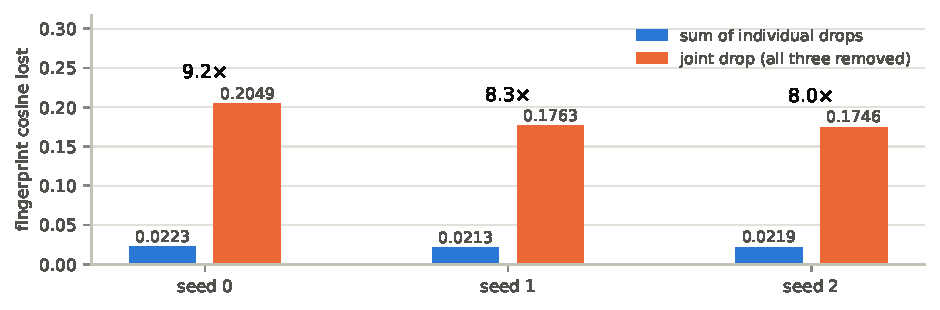
\includegraphics[width=\textwidth]{fig-superadditivity.pdf}
\caption{The NMR block is jointly essential and individually disposable.
Removing HSQC, $^{13}$C and $^{1}$H \emph{together} costs $8.0$--$9.2\times$
more fingerprint cosine than the sum of removing them one at a time.}
\label{fig:superadd}
\end{figure}

\noindent
Structurally this is an interaction-information or Shapley-synergy measure
evaluated on the loss surface rather than on entropies. Its practical reading:
\textbf{any one NMR modality can be reconstructed from the others; all three
cannot.} It also bounds how much weight a single-modality ablation table can
bear --- including the dereplication tables --- since every such number is
measured with the redundant partners still present.

\FloatBarrier
\section{The other redundancy: the fingerprint target}
\label{sec:fpredundancy}

Every ablation number in \S\ref{sec:budget}--\S\ref{sec:redundancy} is
denominated in \emph{fingerprint cosine}. That unit is not neutral, and a
companion analysis measured exactly how far from neutral it is
(\code{Datasets/fp-redundancy/}, MARINA1, checkpoint \code{final1}). Its
findings belong here because they bound how the numbers above should be read
--- and because they are the same phenomenon at the other end of the model.

\subsection{The target carries far less information than its width}

\code{EntropyFPLoader.setup} selects the $16{,}384$-bit fingerprint by ranking
candidate circular substructures on \emph{marginal} binary entropy. Binary
entropy is monotonic in $p$ below $0.5$ and the selected bits are rare (median
presence $0.0009$, $471$ of $518{,}901$ molecules), so ``top-$K$ by entropy''
is exactly ``top-$K$ by frequency''. Nothing in that criterion penalises bits
for being correlated with each other.

They are. For any tree $T$ over the bits,
$H(\text{joint}) \le \sum_i H_i - \sum_{(i,j) \in T} I(i;j)$, and the maximum
spanning tree of the mutual-information graph makes the bound tightest:

\begin{table}[htbp]
\centering
\small
\caption{Realised capacity of the fingerprint. About $0.9\%$ of nominal width
is information --- though still $7.7\times$ what is needed to index the
retrieval set uniquely.}
\label{tab:fpcapacity}
\begin{tabular}{@{}l r@{}}
\toprule
& Bits \\
\midrule
Nominal width & 16{,}384 \\
$\sum_i H_i$ (marginal entropies) & 422.6 \\
$-$ Chow--Liu MST mutual information & 275.3 \\
\textbf{Joint entropy (tightest tree upper bound)} & $\le$ \textbf{147.4} \\
Needed to index the 519K retrieval set & 19.0 \\
\bottomrule
\end{tabular}
\end{table}

\begin{figure}[htbp]
\centering
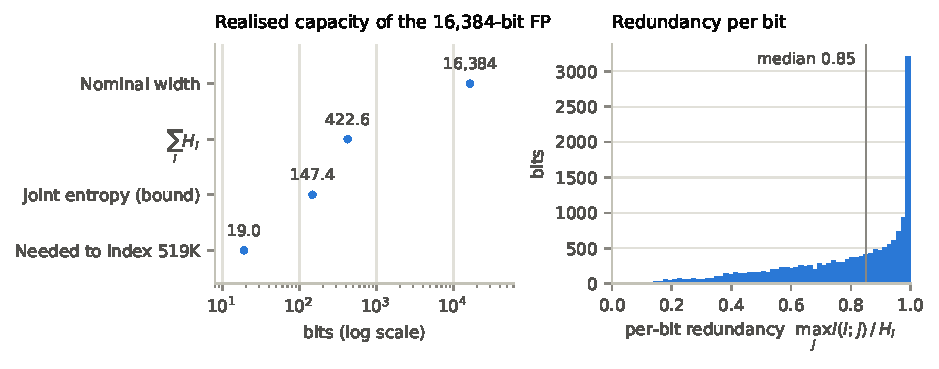
\includegraphics[width=\textwidth]{fig-fp-redundancy.pdf}
\caption{Left: the capacity ladder of Table~\ref{tab:fpcapacity}, on a log
axis --- shown as points rather than bars, since bars on a log scale misstate
proportion. Right: the per-bit redundancy $\max_j I(i;j)/H_i$ over all
$16{,}384$ bits. The mass piled against $1.0$ is bits whose information is
almost entirely duplicated elsewhere in the code.}
\label{fig:fpredundancy}
\end{figure}

\noindent
The structure behind that number:

\begin{itemize}
  \item \textbf{$10{,}608$ of $16{,}384$ bits} have some $j$ with
    $P(i \mid j) = 1$. This is one-way implication ---
    $P(i \mid j) = 1 \iff \operatorname{supp}(j) \subseteq \operatorname{supp}(i)$
    --- so $j$ is a more specific bit that never fires without $i$.
  \item $1{,}695$ bits are \textbf{exact duplicate columns}, collapsing into
    $592$ groups.
  \item Median per-bit redundancy $\max_j I(i;j)/H_i = \mathbf{0.851}$;
    $6{,}731$ bits exceed $0.9$ and $2{,}799$ exceed $0.99$. This is not an
    artifact of rare bits --- the median is still $0.686$ in the
    \emph{most frequent} decile.
  \item By RDKit substructure containment over the $2{,}808$ exact-duplicate
    pairs, $65.7\%$ are \textbf{radius nesting} (the ECFP family itself:
    radius $r$ and $r+k$ around the same environment) and $34.3\%$ are
    \textbf{congeneric series}. The largest duplicate group is 28 bits over 246
    molecules --- gangliosides differing only in ceramide acyl chain length,
    where 28 slots encode ``this is a ganglioside''.
\end{itemize}

\subsection{The redundancy buys nothing}

The natural defence of a redundant code is that it is an error-correcting one:
a model predicting bits from NMR gets several noisy shots at the same target.
That defence fails. Within exact-duplicate groups --- where the target column
is \emph{identical}, so the model sees $g$ copies of one label --- the mean
pairwise correlation of prediction errors is $\rho = 0.973$, against $0.007$
for frequency-matched control pairs. Averaging $g$ such errors gives
\[
  \frac{\operatorname{Var}}{\sigma^2} = \frac{1 + (g-1)\rho}{g} = 0.982,
  \qquad\text{versus } 0.349 \text{ if the errors were independent.}
\]
There is essentially zero error correction. The duplicated bits act as a pure
weight multiplier on their substructure family.

Nor can the waste be reclaimed by fixing the retrieval metric. Holding model
and bits fixed and changing only the similarity to a weighted cosine
$\operatorname{sim}_w(q,r) = \ip{s \odot q}{s \odot r}/(\norm{s \odot q}\,\norm{s \odot r})$
with $s = \sqrt{w}$ gives Table~\ref{tab:reweight}: down-weighting redundant
bits never helps, and past the exact-duplicate null it hurts monotonically in
decorrelation strength.

\begin{table}[htbp]
\centering
\small
\caption{Down-weighting redundant bits at retrieval time, $n = 3{,}000$ test
molecules, paired. Collapsing exact duplicates is a clean null; everything
stronger degrades top-1 monotonically in decorrelation strength.}
\label{tab:reweight}
\begin{tabular}{@{}l l r r l@{}}
\toprule
Scheme & $w$ & Top-1 & $\Delta$ & McNemar $p$ \\
\midrule
uniform (current) & $1$ & \textbf{0.7587} & --- & --- \\
dup & $1/\text{exact-group-size}$ & 0.7597 & $+0.0010$ & 0.55 \\
soft0.99 & $1/\#\text{partners} \ge 0.99$ & 0.7553 & $-0.0033$ & 0.099 \\
soft0.9 & $1/\#\text{partners} \ge 0.9$ & 0.7513 & $-0.0073$ & 0.0021 \\
soft0.7 & $1/\#\text{partners} \ge 0.7$ & 0.7473 & $-0.0113$ & 0.0027 \\
soft0.5 & $1/\#\text{partners} \ge 0.5$ & 0.7307 & $-0.0280$ & $6\times10^{-9}$ \\
idf (control) & $\log(N/\text{count})$ & 0.7230 & $-0.0357$ & $9\times10^{-24}$ \\
\bottomrule
\end{tabular}
\end{table}

\begin{remark}[What the sweep does and does not show]
Reweighting at test time introduces a train/test mismatch independent of the
redundancy question: the model was trained under a uniform-weight loss and its
predictions are calibrated to the redundant code. That the \code{idf} control
hurts about as much as \code{soft0.5} is consistent with mismatch, not
redundancy, driving the degradation. The sweep therefore rules out a
\emph{free} post-hoc win; it does not show that a low-redundancy fingerprint
would underperform. Settling that needs MI-aware bit \emph{selection} and a
retrain.
\end{remark}

\subsection{What this means for the numbers above}

Three consequences for reading \S\ref{sec:budget}--\S\ref{sec:redundancy}.

\begin{enumerate}
  \item \textbf{Absolute drops are in a distorted unit.} Cosine over this
    fingerprint implicitly weights each substructure family by how many
    correlated copies the frequency ranking happened to pick up --- up to 28
    for one ganglioside core. A drop of $0.013$ cosine is therefore \emph{not}
    ``$1.3\%$ of the chemically relevant information''. It is $1.3\%$ of a
    quantity whose weighting is an artifact of bit selection.
  \item \textbf{Rankings are more robust than magnitudes.} Every reweighting
    short of the most aggressive moves top-1 by at most $0.011$, so the
    \emph{ordering} of the five modalities in Table~\ref{tab:budget} is
    unlikely to be a metric artifact --- consistent with its agreement with
    attribution, which does not touch the fingerprint at all.
  \item \textbf{The superadditivity ratio is comparatively insulated.} $S$ is a
    ratio of two cosine drops, so a multiplicative distortion common to
    numerator and denominator partly cancels. This is a heuristic, not an
    invariance --- the joint and individual ablations need not distort
    identically --- but it makes $S \approx 8.5$ a safer number than the
    $0.0218$ and $0.1853$ it is built from.
\end{enumerate}

\noindent
The broader point is the symmetry. \S\ref{sec:redundancy} finds redundancy on
the \emph{input} side: five modalities whose NMR block is $8.5\times$
superadditive, because any one can be reconstructed from the others. This
section finds redundancy on the \emph{output} side: a $16{,}384$-bit target
realising $\le 147.4$ bits. MARINA has substantially fewer effective channels
than nominal ones at both ends, and neither redundancy was designed in --- the
input one is a consequence of $50\%$ modality dropout, the output one of
ranking bits on marginal rather than joint entropy.

\FloatBarrier
\section{Results: refining the budget by depth}
\label{sec:depth}

Theorem~\ref{thm:main} indexes contributions by $(k,\ell)$ but the reported
shares sum over $\ell$. Restoring that index gives two per-block quantities.

\paragraph{Injection} --- the norm of what block $\ell$ wrote, at the moment of
writing, before any later LayerNorm touches it:
\[
  \operatorname{inj}(k,\ell) \;=\; \big\lVert p_{k,\ell} \big\rVert_2
  \qquad\big(\text{and } \lVert f_\ell\rVert_2 \text{ for } k = \code{ffn}\big).
\]
Unsigned, in raw activation-norm units, with no cross-modality normalisation.

\paragraph{Survival} --- the same vector after transport to the output,
projected onto the final direction exactly as in \eqref{eq:share}:
\[
  \operatorname{sur}(k,\ell)
  \;=\; \frac{\ip{T^{\mathrm a}_\ell\, p_{k,\ell}}{\hat q_N}}{\lVert q_N\rVert}.
\]
Signed, dimensionless, and a strict refinement rather than a new measure:

\begin{corollary}[Depth refinement]
\label{cor:refine}
$\displaystyle\sum_{\ell=0}^{N-1} \operatorname{sur}(k,\ell) = \text{share}_k$
for every bucket $k$.
\end{corollary}

\begin{proof}
Immediate from Theorem~\ref{thm:main} and the linearity of
$\ip{\cdot}{\hat q_N}$.
\end{proof}

\paragraph{Retention} --- their ratio,
$\operatorname{ret}(k,\ell) = \operatorname{sur}(k,\ell)/\operatorname{inj}(k,\ell)$:
what one unit of injected norm is worth at the output. Note it folds together
two distinct effects --- attenuation of magnitude by the repeated division by
$\sigma$, and misalignment with $\hat q_N$ --- and cannot separate them, since
the numerator is a signed projection and the denominator an unsigned norm.

\begin{figure}[htbp]
\centering
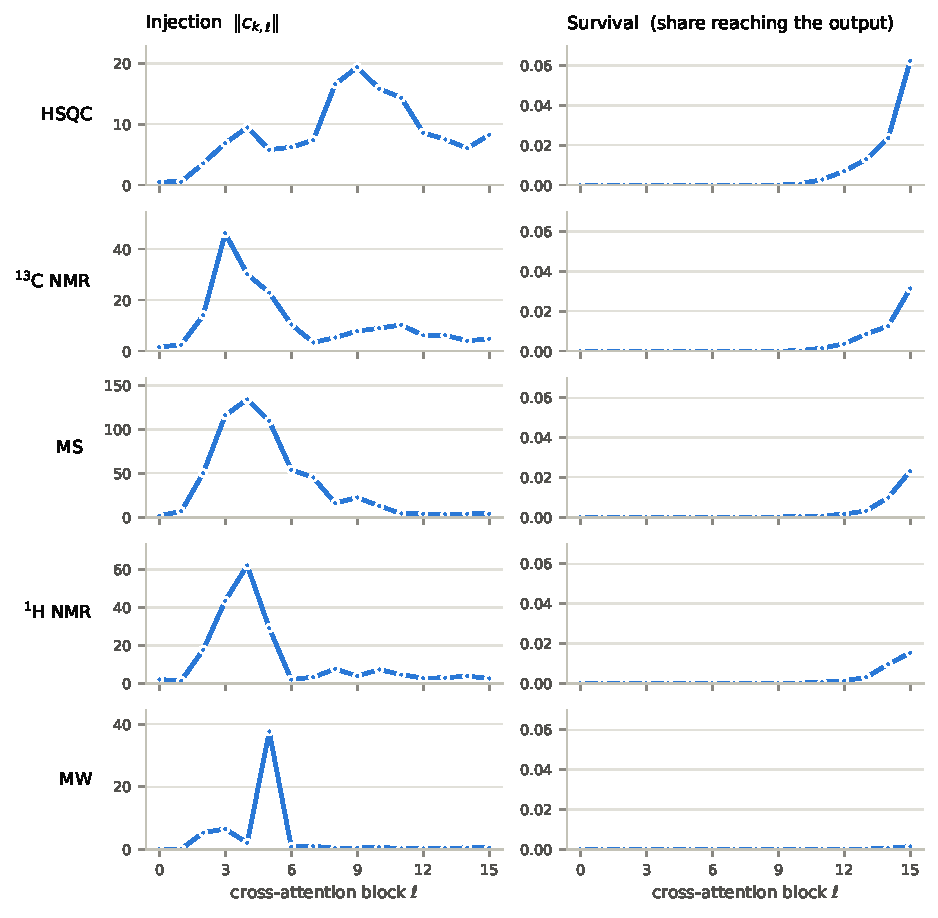
\includegraphics[width=\textwidth]{fig-layer-profile.pdf}
\caption{Where each modality is read, against where that reading survives.
$n = 256$, seed 1. Survival shares one scale across rows because it is a share
of one common budget; injection does not, because a raw activation norm carries
no cross-modality meaning. \textbf{The columns peak at opposite ends of the
stack.} Reading is heaviest at blocks 3--9; essentially none of it reaches the
output, while block 15 alone --- often a smaller write --- delivers most of
what survives.}
\label{fig:layers}
\end{figure}

\begin{table}[htbp]
\centering
\small
\caption{Per-block profile, $n = 256$, seed 1. The last two columns verify
Corollary~\ref{cor:refine} numerically: summing survival over the sixteen
blocks reproduces the aggregate share of \eqref{eq:share} to nine decimal
places. (Shares here are for this $n = 256$ subsample, so they differ slightly
from Table~\ref{tab:budget}'s $n = 23{,}648$ figures.)}
\label{tab:perlayer}
\begin{tabular}{@{}l c r r r r r@{}}
\toprule
& Peak inj. & \multicolumn{2}{c}{At $\ell = 15$} & $\sum_\ell \operatorname{sur}$ & $\text{share}_k$ & $|\text{diff}|$ \\
\cmidrule(lr){2-2}\cmidrule(lr){3-4}
Bucket & block (value) & inj. & sur. & & & \\
\midrule
HSQC & 9\ \ (19.4) & 8.3 & 0.0623 & 0.109428 & 0.109428 & $2.5\times10^{-9}$ \\
$^{13}$C NMR & 3\ \ (46.2) & 4.8 & 0.0315 & 0.058190 & 0.058190 & $2.9\times10^{-10}$ \\
MS & 4\ (134.2) & 4.0 & 0.0231 & 0.038983 & 0.038983 & $6.5\times10^{-10}$ \\
$^{1}$H NMR & 4\ \ (62.2) & 2.5 & 0.0153 & 0.029919 & 0.029919 & $6.4\times10^{-10}$ \\
MW & 5\ \ (37.7) & 0.5 & 0.0014 & 0.002144 & 0.002144 & $7.0\times10^{-11}$ \\
\code{ffn} & 2\ (4816) & --- & --- & 0.712767 & 0.712767 & $1.8\times10^{-9}$ \\
\bottomrule
\end{tabular}
\end{table}

\noindent
The pattern in Figure~\ref{fig:layers} and Table~\ref{tab:perlayer} is
consistent across every modality: \textbf{the block that reads hardest is
never the block that matters}. MS injects $134.2$ at block 4 --- the loudest
read anywhere in the model --- and its survival there is below $10^{-4}$. HSQC
peaks at block 9 with $19.4$ and survives $10^{-4}$; at block 15 it injects
less than half as much, $8.3$, and survives $0.0623$, some $600\times$ more.

The mechanism is the repeated $1/\sigma$ division of Lemma~\ref{lem:ln}. Every
bucket alive at block $\ell$ is rescaled again at every later block, and the
feedforward writes that set $\sigma$ early are enormous: $\code{ffn}$ injects
$4816$ at block 2, two orders of magnitude above any modality's read. Anything
written before that is scaled toward nothing. Retention accordingly rises
roughly geometrically over the last five blocks --- for HSQC, $\times10^3$:
$0.2$, $0.8$, $1.7$, $3.9$, $7.5$.

\begin{remark}[Why this is not yet a conclusion]
Near-zero survival for blocks 0--9 is consistent with two incompatible
stories: the early reads are discarded, \emph{or} they matter through the
feedforward path, whose bucket content depends on $u_\ell$ and hence on
everything read at blocks $\le\ell$. A linear decomposition cannot distinguish
them, and the feedforward path holds $71\%$ of the budget. That is what
\S\ref{sec:suppression} is for.
\end{remark}

\FloatBarrier
\section{Results: attention-depth suppression}
\label{sec:suppression}

A forward hook on each block's \code{MultiheadAttention} suppresses reading in
a contiguous set of blocks; the block still runs its feedforward and
LayerNorms, it just reads nothing. No weights are modified. This is a causal
intervention, so unlike \S\ref{sec:depth} it follows the feedforward path.

\begin{table}[htbp]
\centering
\small
\caption{Cross-attention suppression, single checkpoint
(\code{final1/best.ckpt}), $n = 512$, baseline cosine $0.9546$. A dash means
that $k$ was not run for that direction.}
\label{tab:suppress}
\begin{tabular}{@{}r r r c r r@{}}
\toprule
& \multicolumn{2}{c}{First $k$ blocks} & & \multicolumn{2}{c}{Last $k$ blocks} \\
\cmidrule(lr){2-3}\cmidrule(lr){5-6}
$k$ & cos & drop & & cos & drop \\
\midrule
1 & 0.9546 & 0.0000 & & 0.9178 & \textbf{0.0368} \\
2 & 0.9546 & 0.0000 & & 0.8413 & 0.1133 \\
3 & 0.9546 & 0.0000 & & 0.7611 & 0.1935 \\
4 & 0.9546 & 0.0000 & & 0.6826 & 0.2720 \\
5 & 0.9547 & $-0.0001$ & & --- & --- \\
6 & 0.9544 & 0.0002 & & 0.5049 & 0.4498 \\
8 & 0.9536 & 0.0010 & & 0.2717 & 0.6829 \\
10 & 0.9475 & \textbf{0.0072} & & --- & --- \\
12 & 0.7024 & 0.2523 & & --- & --- \\
14 & 0.4812 & 0.4734 & & --- & --- \\
16 & 0.1771 & 0.7775 & & --- & --- \\
\bottomrule
\end{tabular}
\end{table}

\begin{figure}[htbp]
\centering
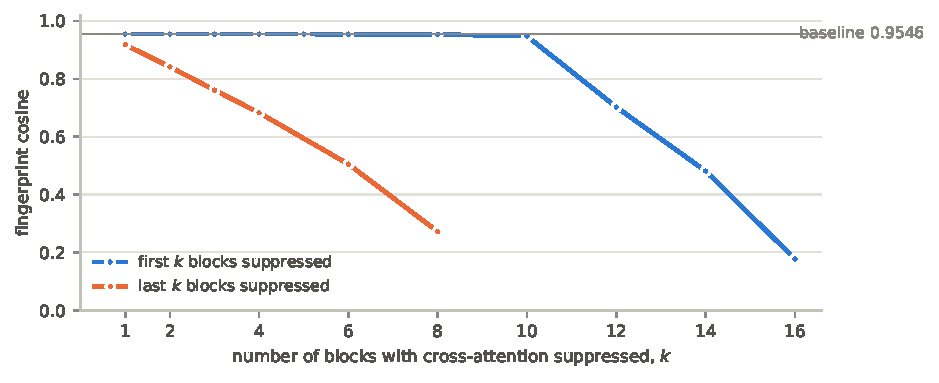
\includegraphics[width=\textwidth]{fig-depth-ablation.pdf}
\caption{The asymmetry is the result. Suppressing cross-attention in the first
ten blocks costs $0.0072$ cosine; suppressing it in the last \emph{one} costs
$0.0368$ --- five times the damage from one block than from ten. The curve
breaks sharply between $k = 10$ and $k = 12$.}
\label{fig:depth}
\end{figure}

\noindent
Table~\ref{tab:suppress} and Figure~\ref{fig:depth} settle the ambiguity left
open in \S\ref{sec:depth}: the early reads are
genuinely discarded, not routed through the feedforward path. Blocks 0--9 of a
16-block stack do nothing useful with their cross-attention in the converged
model. Suppressing the first five is, if anything, very slightly
\emph{beneficial} ($-0.0001$, within noise) --- exactly what one expects of a
read that contributes nothing but numerical jitter.

The practical consequence is a prediction: an 8- or 12-layer model should match
16 layers at lower cost. Two caveats bound how far this result travels. It is a
single checkpoint at $n = 512$, not seed-replicated, whereas the budget of
\S\ref{sec:budget} is three seeds at $n = 23{,}648$; and it used a local
checkpoint copy rather than the three PVC \code{marina-final-run} checkpoints
(baseline cosines agree, $0.9546$ against $0.9548$, but they are not the
identical artifact).

\FloatBarrier
\section{Where exactness ends}

\begin{center}
\begin{tabular}{@{}l l@{}}
\toprule
\textbf{Component} & \textbf{Status} \\
\midrule
span partition (Prop.~\ref{prop:partition}) & exact \\
attention split by source (Prop.~\ref{prop:split}) & exact \emph{given} $\alpha$ \\
value bias $b_V$ & apportioned by attention mass, not isolated \\
LayerNorm transport (Lem.~\ref{lem:ln}) & exact, $\sigma$ frozen at its realised value \\
residual additions & exact \\
$b_O,\ \beta^{(1)},\ \beta^{(2)}$ & exact, in a separate bucket \\
\textbf{feedforward} & \textbf{not decomposable} --- $\mathrm{ReLU}$ \\
$\alpha$ as a function of the input & \textbf{not followed} \\
\bottomrule
\end{tabular}
\end{center}

\medskip
\noindent
The last two entries are the substantive limits. Since
$f_\ell = W_2\,\mathrm{ReLU}(W_1 u_\ell + b_1) + b_2$ admits no exact
source-wise split, the whole vector is assigned to the bucket
$(\code{ffn},\ell)$ --- and that family of buckets absorbs $0.72$ of the total
budget. Crucially, the \emph{content} of the feedforward bucket still depends
on everything read at blocks $\le \ell$, through $u_\ell$. A modality whose
attribution share is near zero may therefore still influence the output
\emph{via} the feedforward path, and this decomposition cannot detect it.

That is not a fixable defect of the accounting. It is the reason a separate,
causal instrument (attention suppression, \code{early\_attn\_ablation.py})
is required. The decomposition tells you what the residual stream is
\emph{made of}; only intervention tells you what it \emph{depends on}.

\end{document}
